\chapter{相关技术概述}
\section{相关算法}
\subsection{K-Shape时间序列聚类算法}
\label{section2.1.1}
K-Shape算法\cite{yang2017k}是一种基于形状的时间序列聚类算法,用于将相似的时间序列分为同一类。其基本思想是通过对时间序列进行自动化预处理和转换,然后使用基
于形态的距离SBD(\textbf{\underline{S}}hped-\textbf{\underline{B}}ased \textbf{\underline{D}}istance)来计算时间序列之间的相似
度,从而实现聚类。K-Shpae使用归一化的互相关系数$NCC_{c}$(Normalized Cross-Correlation Coefficient)来描述两个时间序列的形状相似性。$NCC_{c}$是
一种衡量两个时间序列在不同时刻相似程度的度量方法。通过计算一个序列与另一个序列的滑动版本之间的相似性,我们可以识别它们之间的潜在关系。在时间序列 \( x_t \) 
和 \( y_t \) 中,\( x_t \) 可以通过滑动窗口 \( s \) 来计算与 \( y_t \) 的互相关 \( CC_w(x_t, y_t) \),其中 \( s \) 是滑动窗口的大小,
\( x_t' \) 是 \( x_t \) 的滑动版本。当 \( s > 0 \) 时,\( x_t' \) 是 \( x_t \) 向右滑动 \( s \) 个单位的结果,
即 \( x_t' = (0, \ldots, 0, x_1, x_2, \ldots, x_{m-s}) \);当 \( s < 0 \) 时,\( x_t' \) 是 \( x_t \) 向左滑动 \( |s| \) 个单位
的结果,即 \( x_t' = (x_{-s}, \ldots, x_m - 1, x_m, 0, \ldots, 0) \)。具体表达式如公式\eqref{eq:shift}所示:
\begin{equation}
    x_(s) = 
        \begin{cases} 
        \overbrace{(0, \ldots, 0)}^{|s|}, x_{1+s}, x_2, \ldots, x_{m-s}, & s \geq 0 \\
        x_{1-s}, \ldots, x_{m-1}, x_m, \underbrace{(0, \ldots, 0)}_{|s|}, & s < 0 
        \end{cases}
    \label{eq:shift}
\end{equation}
\( CC_w(x_t, y_t) \) 的计算公式如公式\eqref{eq:NCC1}与公式
\eqref{eq:NCC2}所示。
当 \( w \leq m \) 时,
\begin{equation}
CC_w = \sum_{k=1}^w x'_k \cdot y_{k+m-w}
\label{eq:NCC1}·
\end{equation}
当 \( w > m \) 时,
\begin{equation}
CC_w = \sum_{k=1}^{2m-w} x'_{k-m+w} \cdot y_k
\label{eq:NCC2}
\end{equation}
其中,\( m \) 是序列的长度,\( w \) 是滑动窗口的宽度。这允许我们在不同的时间滞后下计算序列 \( x_t \) 和 \( y_t \) 之间的相似度。
如图\ref{fig:NCC}所示,当$x_t$右移2步时\( CC_w(x_t, y_t) \)达到最大序列对齐。
\begin{figure}[H]
    \centering
    % Requires \usepackage{graphicx}
    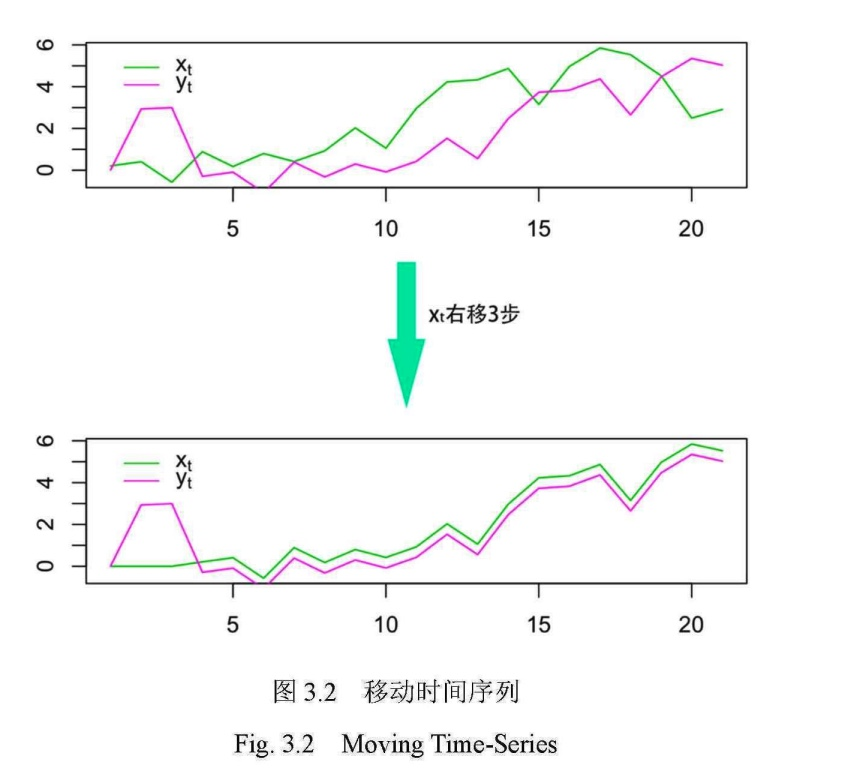
\includegraphics[scale=0.3,angle=0]{figure/NCC.jpg}\\
    \caption{移动时间序列}
    \label{fig:NCC}
\end{figure}
不同的时间序列数据可能在量级上差异巨大,需要对其归一化调整到相同的尺度。归一化是数据预处理中常用的技术,主要用于调整数据集中变量的尺度,使
其具有统一的标准。这通常通过将每个数据点减去平均值并除以标准差来实现,以便转化后的数据集具有零均值(\( \mu = 0 \))和单位方差
(\( \sigma^2 = 1 \))。这种转换被称为标准化或Z得分归一化。对于一个给定的时间序列 \( x_t \),其归一化后的值 \( x_t' \) 可以通过以下
公式计算得出:

\begin{equation}
x_t' = \frac{x_t - \mu}{\sigma}
\label{eq:normal1}
\end{equation}

其中,\( \mu \) 是原始时间序列 \( x_t \) 的均值,\( \sigma \) 是其标准差。这个过程确保了不同的数据集可以在相同的比例上进行比较和分析。K-Shape
算法采用系数归一化$NCC_c = \frac{CC_w(x,y)}{\|x\|\|y\|}$的方式对\( CC_w(x, y) \)进行归一化。互相关序列除以各个序列自的几何平均值。归一化后,
SBD的计算公式如式\eqref{eq:SBD}所示:
\begin{equation}
    SBD(x_t, y_t) = 1 - \max_w \left( \frac{CC_w(x_t, y_t)}{\|x_t\| \cdot \|y_t\|} \right)
    \label{eq:SBD}
\end{equation}
当两段时间序列重合越多,他们形状越相似,$CC_w(x_t, y_t)$就越大。对比所有可能位置的相似度值,取最相似的$max(NCC_c)$,再通过$1-max(NCC_c)$得到
SBD。表明了当两条时间序列越相似时,SBD越小。由于归一化以后的$NCC_c$在[-1,1]之间,因此SBD的值在[0,2]之间。当SBD=0时,意味着两条序列一模一样。
但是用上述方法对序列之间距离做对比时,时间复杂度为$O(m^2)$,当序列长度较长时,复杂度会很高,计算量也会很大。为解决这一问题,作者通过傅立叶变换的
方法,将序列从时域转换为频域再进行比较。此时,离散傅里叶变换(Discrete Fourier Transform, DFT)及其逆变换(Inverse Discrete Fourier Transform, IDFT)发挥了
至关重要的作用。DFT将时域信号转换为频域表示,而IDFT则实现了反向过程,允许序列从频域返回到时域。在K-shape聚类算法中,DFT和IDFT的运用可以描述如下。
给定时间序列 \( x_t \) 和 \( y_t \),首先应用DFT将这些序列转换为它们的频域表示 \( F(x_k) \) 和 \( F(y_k) \)。在频域中,通过简单地把原序列
的DFT结果,应用IDFT,我们可以有效地计算序列间在不同滑动窗口 \( w \) 下的互相关 \( CC_w(x_t, y_t) \)。
离散傅立叶变换和逆变换的数学表达式公式\eqref{eq:DFT}为:
\begin{equation}
    F(x_k) = \sum_{r=0}^{m-1} x_r e^{-\frac{2 \pi i r k}{m}}, \quad k = 0, \ldots, m - 1
    \label{eq:DFT}
\end{equation}
\begin{equation}
    F^{-1}(x_r) = \frac{1}{m} \sum_{k=0}^{m-1} F(x_k) e^{\frac{2 \pi i k r}{m}}, \quad r = 0, \ldots, m - 1
    \label{eq:IDFT}
\end{equation}
根据这些变换,互相关可以通过公式\eqref{eq:ccf}计算:
\begin{equation}
    CC_w(x_t, y_t) = F^{-1}(F(x_t) \times F(y_t))
    \label{eq:ccf}
\end{equation}
通过傅立叶变换的方式计算互相关的算法复杂度为\( O(m \log m) \),这使其计算SBD时在计算性能上十分高效,可以显著加快整个聚类过程。
K-Shape需要在簇内找到最优簇心$c_k^* = [c_1 \quad c_2 \quad \ldots \quad c_m]$使得簇$P_t$内所有序列$x_t$与$c_k^*$的SBD距离总和最小。其
等价的最大化问题为公式\eqref{eq:ck1}。
\begin{equation}
    c_k^* = \arg\min_{c_k} \sum_{x_t \in P_k} SBD(x_t, c_k)
    \label{eq:ck1}
\end{equation}
根据K-Shpae迭代的特性,将公式\eqref{eq:ck1}与公式\eqref{eq:SBD}结合,并将$c_k$标准化,可得到最终的簇心计算公式为式\eqref{eq:ckfin},其中$\mathbf{S} = \sum_{x_t \in P_k} x_t \cdot x_t^T$
\begin{equation}
    c_k^* = \arg\max_{c_k} \frac{c_k^T \cdot \mathbf{S} \cdot c_k}{c_k^T \cdot c_k}
    \label{eq:ckfin}
\end{equation}
此时,问题转化为了经典的瑞利商(Rayleigh Quotient)问题。只要求得矩阵$\mathbf{S}$的最大特征值,$c_k$的解就是$\mathbf{S}$最大特征值对应的特征向量。
\subsection{门控循环单元}
门控循环单元(Gated Recurrent Unit, GRU)[57]是循环神经网络(Recurrent Neural
Network, RNN)的变体。循环神经网络(RNN)是一种专门用于处理序列数据的神经网络。它的内部结构包括一个循环单元,用于存储过去的信息,使网络能够利用之前的信息来处理当前的输入。这种结构允许信息随时间传递,使得RNN特别适用于时间序列数据或任何形式的有序数据。在RNN中,每个节点都接收前一个时间步的输出和当前时间步的输入作为其输入,创建了一个在时间上循环的网络。
原始的RNN在处理长期依赖问题时表现不佳,容易出现梯度消失和梯度爆炸的问题,这使得模型难以从长序列中有效地学习信息。为了解决这个问题,研究者们提出了LSTM(长短期记忆)和GRU(门控循环单元)两种变体,通过加入门控的方式选择性地保留长期依赖。
与传统的RNN相比,LSTM的独特之处在于其内部结构,它包含有三个重要的门控机制:忘记门、输入门和输出门,以及一个持久的细胞状态,这些共同工作以保持和调节信息流。其中忘记门负责决定哪些信息应从细胞状态中移除,这通过观察当前输入和上一个时间步的隐藏状态来决定,帮助网络忘记那些不再重要的信息。
输入门决定哪些新信息将被存储在细胞状态中,使网络能够更新其存储的信息以反映新接收到的重要数据。输出门控制从细胞状态到隐藏状态的信息流,确定下一个时间步的输出应该包含哪些内容。
细胞状态则像一条传送带,横贯整个LSTM结构,只有通过门控制的微小调整,允许信息无阻碍地流过整个链。这种设计使得LSTM能够在长时间间隔内保存状态和记忆,有效避免了传统RNN中常见的梯度消失问题。
GRU是一种与LSTM相似的RNN架构,但结构上更为简化。其旨在解决传统RNN无法有效处理长期依赖问题的同时,减少计算复杂度和模型参数量,从而加快训练速度并减少计算资源需求。
GRU的关键在于它将LSTM中的三个门(忘记门、输入门和输出门)简化为两个门:更新门(Update Grate)和重置门(Reset Grate)。其中更新门决定了从一个状态到另一个状态有多少信息是需要更新的。更新门帮助模型决定在当前状态的信息中保留多少旧信息和加入多少新信息。它类似于LSTM中的忘记门和输入门的结合。
重置门用来决定在计算新状态时应该忽略多少之前的信息。通过这种方式,重置门允许模型抛弃和忘记不重要的信息,有助于捕捉数据中的短期依赖特征。
除了门控机制,GRU中还有一个重要的概念是隐藏状态(Hidden State),它类似于LSTM中的细胞状态和隐藏状态的结合体,但更加简化。隐藏状态在每个时间步被更新,并用于捕获并传递序列中的信息。
与LSTM相比,GRU的优势在于模型结构更简单,这意味着它们需要更少的参数,从而减少了内存消耗,加快了训练速度。LSTM和GRU的结构如图\ref{fig:lstmandgru}所示。
\begin{figure}[H]
    \centering
    \caption{LSTM/GRU结构示意图}
    \label{fig:lstmandgru}
\end{figure}
\subsection{Transformer模型}
在神经网络发展过程中,面对计算性能的限制和模型复杂度的增加,信息过载成为了一个突出问题。为应对这一挑战,业界借鉴人脑处理信息的策略,提出了注意力机制(Attention)。这一机制通过集中关注对当前任务更为关键的信息,同时忽略不相关的数据,从而提高神经网络的处理效率和性能。

注意力机制的核心原理是对信息进行加权处理,增加关键信息的重量,减少无关信息的影响。这一机制通过三种向量实现:查询向量$\mathbf{Q}$(Query)、关键向量$\mathbf{K}$(Key)和值向量$\mathbf{V}$(Value)。其中,查询向量代表与当前任务相关的需求,关键向量代表数据的关键属性,两者相互作用生成一个注意力分布,进而决定值向量中哪些信息是当前步骤需要关注的。

Transformer模型是一种完全基于注意力机制的架构,由Google公司开发\cite{vaswani2023attention}。它能够进行并行计算,有效捕捉长距离的依赖关系。该模型采用了编码器-解码器(Encoder-Decoder)结构,整个流程包括数据输入、编码处理、解码处理和最终输出四个主要部分,能够处理各种序列到序列的任务。

(1)数据输入

序列数据首先通过输入嵌入(Input Embedding)转换为嵌入向量,以此表示数据中的每个元素。随后,为了让模型能够识别序列中每个元素的位置,会为每个嵌入向量增加位置编码PE(Positional Encoding)。这样可以保持序列的顺序信息。
PE的计算过程如公式\eqref{pos2i}和公式\eqref{posi}所示。
\begin{equation}
    PE(pos, 2i) = \sin\left(\frac{pos}{10000^{2i/d_{\text{model}}}}\right)
    \label{pos2i}
\end{equation}
\begin{equation}
    PE(pos, 2i+1) = \cos\left(\frac{pos}{10000^{2i/d_{\text{model}}}}\right)
    \label{posi}
\end{equation}
式中,\textit{pos} 代表序列中某一数据点在整个序列中的绝对位置,\(d_{\text{model}}\) 代表数据的嵌入向量维度,而 \textit{i} 表示向量中的具体维度位置。此外,\(2i\) 和 \(2i + 1\) 分别代表向量中的偶数和奇数位置维度。这种表示方法有助于在位置编码过程中区分不同位置的数据点。

(2)Encoder

在Transformer模型的编码器中,已处理的输入数据以向量形式通过多头注意力机制,随后结合残差连接和层归一化操作(统称为Add\&Norm),以及通过前馈神经网络进行进一步处理。这一系列步骤旨在增强模型对不同输入数据间关系的理解,并提高模型的学习能力及其对序列数据的处理效率。
其中注意力机制的计算过程如公式\eqref{tranatten}所示。
\begin{equation}
    \text{Attention}(Q,K,V) = \text{softmax}\left(\frac{QK^T}{\sqrt{d_k}}\right)V
    \label{tranatten}
\end{equation}
在该文中,\(\mathbf{Q}\)、\(\mathbf{K}\)和\(\mathbf{V}\)分别是输入数据\(\mathbf{X}\)与相应的权重矩阵\(\mathbf{W^Q}\)、\(\mathbf{W^K}\)和\(\mathbf{W^V}\)相乘后得到的向量。这里,\(d_k\)表示向量\(\mathbf{K}\)的维度。softmax归一化指数函数被应用于这些向量的乘积,以将它们映射到一个概率分布上,其值位于区间[0,1]之内,并且所有数值的和为1。
多头自注意力层(MHSA)通过将查询、键和值向量分割成h个较小的子向量组,每组进行独立的自注意力计算,然后将这些结果拼接起来。这种方法不仅减少了计算量,还允许模型在不同的表示子空间中捕捉信息,增强了模型理解全局特征互相关性的能力。
其表达式如式\eqref{trasmuti}所示。
\begin{equation}
    \begin{aligned}
        \text{MultiHead}(Q, K, V) = \text{Concat}(head_1, \ldots, head_h)W^Q \\
        \text{where } head_i = \text{Attention}(QW_i^Q, KW_i^K, VW_i^V)
        \label{trasmuti}
    \end{aligned}
\end{equation}
通过使用一组不同的权重矩阵\(W^Q\)、\(W^K\)和\(W^V\)来生成多组查询向量\(\mathbf{Q}\)、键向量\(\mathbf{K}\)和值向量\(\mathbf{V}\)。每一组的这些向量相互作用,分别产生一个输出矩阵\(\mathbf{Z}\)。最终,这些输出矩阵\(\mathbf{Z}\)被拼接成一个更大的矩阵,以获得综合的信息表达。   
Add\&Norm操作包括两个步骤:首先是残差连接,它将多头注意力的输出\(\mathbf{Z}\)矩阵与输入\(\mathbf{X}\)矩阵相加;其次是归一化,使用层归一化(Layer Normalization)技术对加和后的结果进行标准化,确保数据在一个合理的范围内。
前馈神经网络的计算过程如式\eqref{ffn}所示。
\begin{equation}
    \text{FFN}(x) = \max(0, xW_1 + b_1)W_2 + b_2
    \label{ffn}
\end{equation}
x代表从多头注意力机制得到的输出\(\mathbf{Z}\)矩阵。这个矩阵首先通过一个线性变换过程,然后应用ReLU激活函数进行非线性转换,筛选重要的信号。最后,这个过程通过另一个线性变换完成,产生最终的输出。

(3)Decoder 

Decoder和Encoder的计算原理基本相同,但Decoder增加了掩码多头注意力机制,这一机制通过引入掩码(mask)来修改多头注意力计算过程。其中,padding mask用于处理不同长度的序列,保证数据对齐,而sequence mask防止Decoder提前看到未来的信息,确保每个位置只能依赖于它之前的位置,从而保护序列数据的时序完整性。

(4)输出

从Decoder接收的输入数据首先经历一次线性变换,然后通过softmax函数进行处理,最终输出预测结果。